\documentclass[prl,twocolumn]{revtex4-1}

\usepackage{graphicx}
\usepackage{color}
\usepackage{latexsym,amsmath}
\usepackage{amsfonts}
\usepackage{caption}
\usepackage{siunitx}
\usepackage{physics}

\definecolor{linkcolor}{rgb}{1.0,0.647,0.0} %hyperlink
\usepackage[pdftex,colorlinks=true, pdfstartview=FitV, linkcolor= linkcolor, citecolor= linkcolor, urlcolor= linkcolor, hyperindex=true,hyperfigures=true]{hyperref} %hyperlink%

\usepackage{enumitem}
\setlist[itemize]{leftmargin=*}


\setcounter{secnumdepth}{2}

\renewcommand{\thesection}{\arabic{section}}
\renewcommand{\theequation}{\thesection.\arabic{equation}}

\makeatletter
\@addtoreset{equation}{section} % Reset equation counter at each section
\makeatother

\begin{document}

\title{Quantum Optics and Laser, Lab5 - Quantum key distribution}


\author{Calandra Buonaura Lorenzo}

\date{\today}


\begin{abstract}
In this experiment, we explore a quantum key distribution (QKD) protocol based on the 3-states 1-decoy efficient BB84 scheme. This protocol builds upon the standard BB84 protocol, enhancing its security by introducing decoy states, which are used to estimate the single-photon contribution to the transmission and provide a means to detect potential eavesdropping attempts, particularly photon number splitting (PNS) attacks. The experiment focuses on understanding the operation of this protocol, the role of decoy states in ensuring security, and the methodology for detecting eavesdropping based on the comparison of detection probabilities for signal and decoy states.

\end{abstract}

\maketitle

\section{Introduction}
\label{sec:intro}
This experiment regards Quantum Key Distribution (QKD), which represents a breakthrough in secure communication, as it uses the fundamental principles of quantum mechanics to guarantee the confidentiality of exchanged information. The protocol investigated in this experiment is based on the BB84 scheme, a widely studied and implemented QKD protocol introduced by Bennett and Brassard in 1984. This protocol encodes information in non-orthogonal quantum states and employs random basis choices for state preparation and measurement, ensuring that any attempt at interception by Eve will disrupt the transmission, making eavesdropping detectable.

In particular, this study focuses on the enhanced version of the BB84 protocol called the 3-states 1-decoy efficient BB84 protocol. This modification integrates decoy states to improve security by allowing Alice and Bob to detect and mitigate sophisticated attack; in this variant, Alice and Bob can monitor the transmission statistics and estimate the single-photon contribution, which is critical for generating a secure key.

The purpose of this experiment is to provide a comprehensive analysis of how the 3-states 1-decoy efficient BB84 protocol operates, focusing on the role of decoy states in enhancing the security of the transmission. Through this experiment, we aim to demonstrate the effectiveness of decoy states in preventing eavesdropping and ensuring the security of key generation, even in the presence of potential adversaries.

\section{Theoretical Framework}
This experiment is a straightforward implementation of a Quantum Key Distribution (QKD) protocol, in particular of the 3-states 1-decoy efficient BB84 protocol.

\subsection{Introduction to QKD}
\label{sec:QKD}
QKD is a cryptographic method that enables two parties, commonly referred to as Alice and Bob, to generate a shared secret key using the principles of quantum mechanics. Unlike classical cryptography, whose security most of the times relies on computational complexity, QKD leverages quantum states, such as photons, to encode information. Due to the no-cloning theorem and the disturbance caused by measurement, any eavesdropping attempt by a third party (Eve) introduces detectable errors in the communication, which allows Alice and Bob to identify and mitigate potential security breaches during the key generation process.

The protocol we are considering in this case is a prepare-and-measure protocol, which requires a quantum channel to transmit the information, which is then measured. These QKD protocols consider that the two legitimate parties have two communication channels available; the first is the quantum channel, in which the sender sends qubits (we consider polarized photons), after \textit{preparing} them (encoding), to Bob, who then \emph{measures} them (decoding). We must notice that this is a one-way transmission and we are not inserting any restriction whatsoever on the possibility that Eve is performing eavesdropping of any kind (we suppose that an attack in this part is possible, we want to build a communication that can detect if an attack has been performed).
The second communication channel is a classical two-way authenticated channel (for example the telephone), in which classical information is exchanged; authenticated means that the legitimate parties are sure that they are communicating with each other and not sending the information to a third party. In this channel Eve is only able to read the information, but not to retain or modify it in any way.

\subsection{BB84 protocol}
The BB84 protocol, introduced by Bennett and Brassard in 1984, was the first practical QKD protocol and remains one of the most widely studied schemes. By encoding information in non-orthogonal quantum states and using random bases for preparation and measurement, the BB84 protocol ensures that any interception of the quantum channel results in detectable anomalies~\cite{pap1}.

\subsubsection{State preparation}
For each photon, Alice randomly selects one of the two available bases, $X$ or $Z$, to encode the quantum state. These basis represent the possible polarizations of our photons, and are also called \textit{diagonal} and \textit{rectilinear} basis, respectively (see Figure~\ref{fig:basis_2}). In particular, we have that $Z = \{ \ket H, \ket V\}$ and $X = \{ \ket+, \ket-\}$, where the conversion between the two bases is given by:
%
\begin{equation}
    \ket + =\frac{\ket V + \ket H}{\sqrt{2}}, \qquad \qquad \ket - =\frac{\ket V - \ket H}{\sqrt{2}}.
\end{equation}
%
The choice of basis and intensity level is recorded for later comparison with Bob's measurements, but it's not transmitted with the message, so Bob has no idea which basis has been used for encoding the message.


\begin{figure}
    \centering
    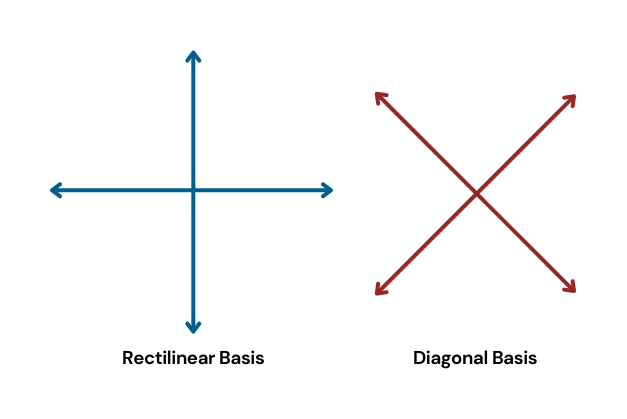
\includegraphics[width=\linewidth]{Images/basis (2).png}
    \caption{Bases used for the state preparation in the BB84 protocol (rectilinear = $Z$ and diagonal = $X$).}
    \label{fig:basis_2}
\end{figure}



\subsubsection{Transmission}
Alice transmits the prepared states through a quantum channel to Bob; in order to do this, it's necessary to encode the message in bits, which can be later decoded. The encoding usually follows the convention depicted by Figure~\ref{fig:basis_1} and presented in Table~\ref{tab:encoding}. As we can see a $0$ in the message string can be translated both to $\ket H$ and $\ket +$, depending on which basis does Bob use for measurement.


\begin{table}[!b]
    \begin{center}
    \begin{tabular}{c|c|c}
        &\textbf{Basis $Z$}& \textbf{Basis $X$}\\
        \hline
        \hline
        \textbf{Bit 0} & $\ket H$ & $\ket +$\\
        \hline
        \textbf{Bit 1} & $\ket V$ & $\ket -$ \\
        \hline
    \end{tabular}
    \caption{Convention used in order to communicate the binary message.}
    \label{tab:encoding}
    \end{center}
\end{table}

\subsubsection{Measurement}
\begin{figure}
    \centering
    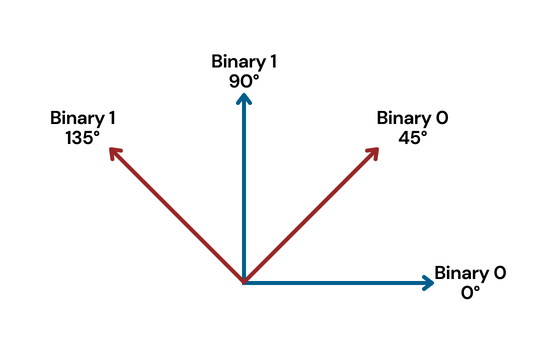
\includegraphics[width=\linewidth]{Images/basis (1).png}
    \caption{Bit - state correspondence used for translating the encoded state in a bit sequence.}
    \label{fig:basis_1}
\end{figure}
Upon receiving the photons, Bob randomly chooses one of the two bases, $X$ or $Z$, for measurement. The outcomes are recorded, and the quantum bit error rate (QBER) is calculated as:
\begin{equation}
\text{QBER} = \frac{\text{\# of erroneous detections}}{\text{\# of detections}}.
\end{equation}
The QBER provides a metric for assessing the presence of eavesdropping and the overall quality of the transmission (which depends on the physical imperfections of the channel and noise of the equipment).

\subsection{Decoy states}
\label{sec:decoy}
The protocol we are considering in this case is a bit different from the presented BB84 protocol, because it leverages decoy states (it's called 3-state 1-decoy efficient BB84 protocol~\cite{pap2}); this integration enhance the security of the protocol, making it robust against sophisticated attacks, including photon number splitting (PNS) attacks.

\subsubsection{Principle of decoy states}
The considered protocol allows for encoding only in 3 states (in our case we have $Z = \{ \ket H, \ket V\}$ and $X = \{ \ket+\}$) and adds a decoy state for enhancing security. Decoy states are not used for key generation and they are indistinguishable from signal states except in intensity (signal = high intensity, decoy = low intensity). By introducing decoy states, the protocol enables the sender and receiver to monitor the transmission statistics and detect potential eavesdropping attempts: specifically, decoy states allow for the estimation of the single-photon contribution to the transmission, which is critical for secure key generation.

\subsubsection{Detection probability}
The detection probability $Q_h$ for the high-intensity states (signal) is expected to be greater than $Q_l$ for the low-intensity states (decoy), as high-intensity pulses contribute additional multi-photon detections. This relationship can be expressed as:
$$
Q_h > Q_l.
$$

\subsubsection{Role of decoy states in eavesdropping detection}

The decoy states are particularly useful for detecting and mitigating \textit{photon number splitting (PNS)} attacks, which are a common threat in quantum key distribution protocols. In a PNS attack, an eavesdropper could intercept multi-photon pulses and split off one photon, measuring it, while keeping the others to learn about the key without disturbing the signal transmission. This would lead to a decrease in the efficiency of key generation and an increase in error rates.

By introducing decoy states, Alice and Bob can compare the detection rates for signal states and decoy states. The decoy states, being of lower intensity, are much less likely to contain multiple photons, so they provide a way to estimate how many multi-photon events have occurred in the signal transmission. If the detection rate for the decoy states is higher than expected, it could indicate that Eve is attempting a PNS attack.


\section{Apparatus}
The experimental setup used for this experiment is presented in Figure~\ref{fig:setup}. As we can see, from a first look, we are not able to tell much about what's going on, so we must explain with a bit more detail what each component does:


\begin{figure}[!b]
    \centering
    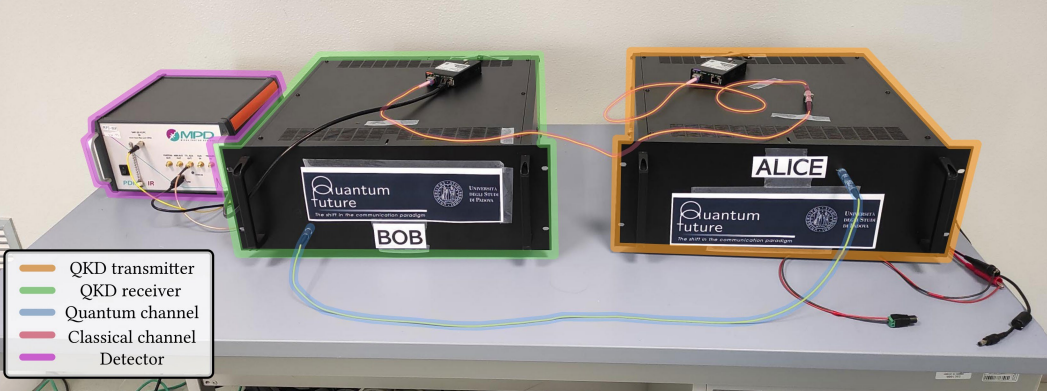
\includegraphics[width=\linewidth]{Images/setup.png}
    \caption{Experimental setup, featuring Alice and Bob boxes, as well as the decoder and optical fibers.}
    \label{fig:setup}
\end{figure}

\begin{itemize}
    \item \textbf{Alice's module (QKD Transmitter)}: Marked in orange, this unit represents Alice's setup. Inside the box, Alice's module includes a quantum source that generates the quantum states (laser producing coherent pulses). The quantum source is coupled with a modulator that encodes the quantum information (photon polarization states), according to the chosen basis. The encoded states are then sent through an optical fiber to Bob via the quantum channel. A key aspect of Alice's module is its ability to generate decoy states at low intensity to enhance security and prevent eavesdropping. 

    \item \textbf{Bob's module (QKD Receiver)}: Marked in green, Bob's unit is the receiver in the QKD setup. The module consists of a random basis selector, which is used to randomly choose between different measurement bases. Then, Bob measures the incoming quantum states transmitted by Alice using photon detectors, which can measure polarization. After measurement, Bob communicates with Alice over the classical channel to compare the selected bases, correct errors, and reconcile the key.
    
    \item \textbf{Quantum channel}: Represented by the blue cable, the quantum channel carries the photons between Alice and Bob. This channel is susceptible to potential eavesdropping or loss due to environmental noise (in our case only this). In a practical setup, indeed, the channel may experience attenuation and other imperfections that affect the transmission efficiency.

    \item \textbf{Classical channel}: Represented by the orange cable, this channel represent the classical communication between Alice and Bob. It is used for tasks such as basis reconciliation, where Alice and Bob compare their choice of bases to determine which bits can be kept for the final key. Additionally, the classical channel is essential for error correction, where discrepancies in the received quantum states are resolved through classical algorithms (e.g., syndrome decoding), and for privacy amplification, which further secures the final key by reducing information leakage. Unlike the quantum channel, the classical channel is typically public (as explained in Section~\ref{sec:QKD}), but its security is ensured by the quantum key distribution protocol.

    \item \textbf{Detector}: Marked in purple, the detector module is connected to Bob's setup; this unit is the one  responsible for detecting and measuring the quantum states received through the quantum channel. The detection efficiency is a crucial factor in the overall performance of the QKD system, and it impacts both the key generation rate and the security of the protocol.
\end{itemize}

The data are then passed in a computer for recording and analysis; the data are stored in 8-bit strings with a specific encoding for each state, in order to be able to reconstruct the signal.

\section{Results}
We have two available datasets so we can compare the results from the two of them. We start analyzing the probability of encoding or decoding in the different bases, then proceed studying the QBER of the channel.

\subsection{Basis choice}
Analyzing the encoding and the decoding probabilities of the two datasets, we find the results presented in Table~\ref{tab:encoding} and in Table~\ref{tab:decoding}, respectively. We can clearly see that, for both sets, most of the times the chosen encoding basis is $Z$ (9 time out of 10). On the other end, the decoding probabilities are roughly equal, with a bit more predominance of the $X$ basis; from this initial observation, we can deduce that the error in the system will be pretty high.

\begin{table}[!h]
    \centering
    \begin{tabular}{c|c|c}
         & Set 1 &  Set 2\\
         \hline
         \hline
        $P(X)$ &  0.1021 & 0.0946\\
        \hline
        $P(Z)$ &  0.8979 & 0.9054\\
    \end{tabular}
    \caption{Encoding probabilities.}
    \label{tab:encoding}
\end{table}


\begin{table}[!h]
    \centering
    \begin{tabular}{c|c|c}
         & Set 1 & Set 2\\
         \hline
         \hline
        $P(X)$ & 0.5327 & 0.5424\\
        \hline
        $P(Z)$ & 0.4673 & 0.4576\\
    \end{tabular}
    \caption{Decoding probabilities.}
    \label{tab:decoding}
\end{table}


\subsection{Conditional probabilities}
\begin{table}[!b]
    \centering
    \begin{tabular}{c|c|c}
         & Set 1 & Set 2\\
         \hline
         \hline
        $P(D|D)$ & 0.5463 & 0.3664 \\
        \hline
        $P(H|D)$ & 0.2444 & 0.2765 \\
        \hline
        $P(V|D)$ & 0.2012 & 0.1937 \\
        \hline
        $P(A|D)$ & 0.0079 & 0.1633 \\
        \hline
        \hline
        $P(D|H)$ & 0.3300 & 0.1691 \\
        \hline
        $P(H|H)$ & 0.4367 & 0.4310 \\
        \hline
        $P(V|H)$ & 0.0099 & 0.0414 \\
        \hline
        $P(A|H)$ & 0.2233 & 0.3584 \\
        \hline
        \hline
        $P(D|V)$ & 0.2177 & 0.3006 \\
        \hline
        $P(H|V)$ & 0.0047 & 0.0472 \\
        \hline
        $P(V|V)$ & 0.4896 & 0.3884 \\
        \hline
        $P(A|V)$ & 0.2877 & 0.2635 \\
    \end{tabular}
    \caption{Conditional probabilities.}
    \label{tab:cond_probs}
\end{table}

We can then analyze the conditional probabilities, where we study the probability of receiving a specific state, given the transmitted state (given the basis chosen by Alice). From the results presented in Table~\ref{tab:cond_probs}, we see that the conditional probability of measuring state $x$ given that Alice transmitted state $x$ is always the highest for all the $x$ states that Alice can encode. At the same time, when choosing the correct basis, Bob decodes the correct state with a very high probability (for example $P(V|V)=0.4896$ against $P(H|V)=0.0047$, where we can have a bit of error due to noise). For the second dataset this behaviour is a bit less pronounced.


\subsection{QBER}
We can now proceed studying the error probabilities; this time we must consider the probability of detecting a state different from the expected one. Table~\ref{tab:QBER} sums up different error probabilities for both sets: from the first tree lines we obtain the error probability fixed a transmitted state, while in the last two we fix that A and B choose the same basis (so this is only error due to noise or a potential eavesdropper). It's obvious that if we fix that A and B choose different basis the error probability tends to 1 for both sets.

We clearly see that in general the second set presents more error; in particular we have that $P(a\neq b|A=X, B=X) = 0.1633$ is a very high error even though the basis is the same. Thus, we should exclude the second set for key generation. 

\begin{table}[!h]
    \centering
    \begin{tabular}{c|c|c}
            & Set 1 & Set 2 \\
            \hline
            \hline
        $P(a\neq b|a=H)$   &   0.5632  & 0.5689 \\
        \hline
        $P(a\neq b|a=V)$   &   0.5103  & 0.6115 \\
        \hline
        $P(a\neq b|a=D)$   &   0.4536  & 0.6335 \\
        \hline
        $P(a\neq b|A=X, B=X)$ & 0.0079 & 0.1633 \\
        \hline
        $P(a\neq b|A=Z, B=Z)$ & 0.0146 & 0.0886 \\
        \hline
    \end{tabular}
    \caption{Error probabilities.}
    \label{tab:QBER}
\end{table}

\subsection{Decoy states}
Finally we can have a look at the decoy states: Table~\ref{tab:decoy} sums up the decoy state probabilities of being in the high and low state. For both sets, we have that the the decoy state is most of the time in the high state, as expected (see Section~\ref{sec:decoy}). Thus we can conclude that in this transmission no eavesdropper tampered the result, as expected.


\begin{table}[!h]
    \centering
    \begin{tabular}{c|c|c}
         & Set 1 & Set 2\\
         \hline
         \hline
        $P(\text{High})$ & 0.8892 & 0.8900\\
        \hline
        $P(\text{Low})$ & 0.1108 & 0.1100\\
    \end{tabular}
    \caption{Decoy probabilities.}
    \label{tab:decoy}
\end{table}


\subsection{Perfect channel}
Finally, et us consider a perfect channel that does not introduce any errors, meaning:

$P(a = b|A = B) = 1$ and $P(b = D|A = Z) = P(b = A|A = Z) = P(b = H|A = X) = P(b = V|A = X) = 0.5$.

Suppose that an eavesdropper intercepts the photons along the channel fiber and measures with the same probabilities as Bob in the basis $E = \{X, Z\}$. After the measurement, the eavesdropper sends the state $e$ measured by them to Bob. 

What's the QBER in this case? We analyze the QBER experienced by Alice and Bob in this intercept-and-resend attack by considering two main cases: $A = B$ and $A \neq B$.

\subsubsection{Case $A = B$}

This can be further divided into two subcases:
\begin{itemize}
    \item When $A = B = E$, Eve does not introduce any error, as they use the same basis as Bob. Thus, $P(a = b|A = B) = 1$ and $P(a \neq b|A = B) = 0$.
    \item When $A = B \neq E$, Eve uses a different basis. This projects the state onto one of the possible states of the other basis, and for Bob, it is equivalent to using the wrong basis. Consequently, $P(b \neq a|A = B \neq E) = P(b \neq a|A \neq B) = 0.5$.
\end{itemize}

The total QBER for $A = B$ is then:
$$
QBER(A = B) = 0.5 \cdot 0.5 = 0.25.
$$

\subsubsection{Case $A \neq B$}
This can be further divided into two subcases:
\begin{itemize}
    \item When $A \neq B = E$, Eve uses a different basis, projecting the state onto one of the possible states of the other basis. Bob uses the same basis as Eve, so he always obtains the same result as Eve. Thus, $P(a \neq b|A \neq E = B) = 0.5$.
    \item When $A = E \neq B$, Eve introduces no additional error, and $P(b \neq a|A = E \neq B) = 0.5$.
\end{itemize}

The total QBER for $A \neq B$ is then:
$$
QBER(A \neq B) = 0.5 \cdot 0.5 + 0.5 \cdot 0.5 = 0.5.
$$

\subsubsection{Total QBER}

The total QBER is the average of the two cases and substituting the values:
\[
QBER_{\text{TOT}} = \frac{0.25 + 0.5}{2} = 0.375.
\]

The total QBER is $37.5\%$, which exceeds the acceptable threshold of $11\%$ (as reported in~\cite{pap3}). Therefore, the protocol successfully detects Eve's attack due to the abnormally high QBER; as a result, Alice and Bob would abort the key generation process, preventing Eve from compromising their security.


\section{Conclusions}
The analysis of encoding and decoding probabilities reveals a clear bias toward the $Z$-basis in encoding, with probabilities $P(Z) = 0.8979$ and $P(Z) = 0.9054$ for the two datasets, respectively. Decoding probabilities are more balanced but slightly favor the $X$-basis, leading to a higher error rate. 

Conditional probabilities show that the correct state is most likely decoded when the transmitted and received bases match. However, errors due to noise or mismatched bases are evident, particularly in the second dataset, which shows significantly higher QBER values. Error probabilities further confirm this trend, indeed, with $P(a \neq b|A=X, B=X) = 0.0079$ for the first set but a much higher $0.1633$ for the second. The high QBER of the second dataset indicates it is unsuitable for secure key generation.

Finally, the analysis of decoy states confirms that the majority of photons are in the high state, suggesting no significant tampering or eavesdropping. However, the presence of high errors in the second dataset emphasizes the need for careful selection of transmission channels to ensure secure communication.

\section{Code}
All the data and the code for the data analysis can be found in this public Github repository: \href{https://github.com/Kallo27/QOL/tree/main/Lab5}{https://github.com/Kallo27/QOL/tree/main/Lab5}

\begin{thebibliography}{99}
\bibitem{pap1}
Charles H. Bennett and Gilles Brassard, \textit{Quantum cryptography: Public key distribution and coin tossing}, Proceedings of IEEE International Conference on Computers, Systems and Signal Processing (1984).

\bibitem{pap2}
Davide Rusca, Alberto Boaron, Fadri Grünenfelder, Anthony Martin, and Hugo Zbinden, \textit{Finite-key analysis for the 1-decoy state QKD protocol}, Appl. Phys. Lett. 112, 171104 (2018).

\bibitem{pap3}
Peter W. Shor and John Preskill, \textit{Simple Proof of Security of the BB84 Quantum Key Distribution Protocol}, arXiv:quant-ph/0003004v2 (2000).

\end{thebibliography}

\end{document}